\section{Signals, Conditioning and Output Constants}

Throughout the controller, various input signals require conditioning and certain output values must be chosen.
The MOSFET transistors used in the H-bridge motor controller and magnet control circuit are driven directly by the DAC.
A 0-9 Volt range was used in an effort to ensure crisp switching. %This is vague and WRONG.
As described in section \ref{sec:voltagecontrol}, the actual motor terminal voltage is measured and used in a feedback loop for error correction. 
A differential ADC was connected across the terminals and passed through a low pass filter to account for digital nature of PWM as described in section \ref{sec:filters}.

The encoder output also required simple processing to determine motor speed and position (in radians), both before and after the gearbox, and the back EMF generated.
The Simulink block diagram responsible for this processing may be seen in Figure \ref{fig:simulinkencoder}.
Encoder gain is given by equation \ref{eq:encodergain} and $K_b$ is provided by the motor datasheet. 
After various unit conversions, it was was found to be $K_b = 0.02424 \frac{V}{rad/s}$.

\begin{figure}[htp]
    \centering
    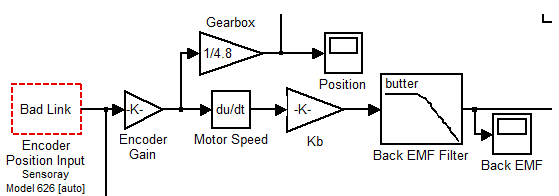
\includegraphics[scale=0.75]{images/Conditioning.PNG}
    \caption{Encoder Conditioning}
    \label{fig:simulinkencoder}
\end{figure}

\begin{equation}
	\label{eq:encodergain}
	K_{encoder} = {\frac {2\,\pi\,{\frac {rads}{revolution}}}{500\,{\frac {slots}{disk}}\times2\,{\frac {pulses}{slot}}\times2\,disks}}
\end{equation}
